% Progress report. Compile from this folder:  pdflatex progress_report && pdflatex progress_report
% Figures are read from ../results/figs/ ; numbers in results_section.tex are generated by scripts/make_tex.py.
\documentclass[conference]{IEEEtran}
\usepackage{amsmath,amssymb}
\usepackage{graphicx}
\usepackage{algorithm}
\usepackage{algpseudocode}
\usepackage{cite}
\usepackage[hidelinks]{hyperref}

\begin{document}

\title{Squint-Free Multi-Beam True-Time-Delay Beamforming with an Approximate Delay Vandermonde Matrix: Reproduction and Physical Evaluation}

\author{\IEEEauthorblockN{[Your Name] (EE24BTECH11220)}
\IEEEauthorblockA{EE3140 Course Project, Department of Electrical Engineering\\
Indian Institute of Technology Hyderabad}}

\maketitle

\begin{abstract}
A wideband antenna array steered by phase shifters points its beams in different directions at different frequencies (beam squint). True time delay (TTD) removes squint, but forming $N$ simultaneous TTD beams directly needs $(N-1)^2$ delay/gain blocks. Perera \emph{et al.}~\cite{perera2025} factorize the $N$-beam delay Vandermonde matrix (DVM) into sparse stages and approximate its FFT stages with a multiplierless transform (ADVM). We reproduce the exact and approximate algorithms in Python and map every matrix stage to an RF component. We then evaluate the result as a physical 16-element array over 5--10~GHz. With TTD, every beam keeps full gain toward its target across the octave. A phase-shifter array is within 3~dB of ideal for only 41\% of the band and delivers about 60\% of ideal link capacity at 20~dB SNR. The exact factorization builds the same 16 beams with 30 delay lines (2.3~m) instead of 225 (27~m). The paper's operation counts are reproduced exactly. ADVM, however, shows a 5.3~dB sidelobe penalty and $1.7^\circ$ of residual squint, larger than reported.
\end{abstract}

\section{Introduction}

\subsection{The physical problem}
An $N$-element uniform linear array with spacing $d$ forms a beam towards angle $\theta$ when the signal of element $l$ is delayed by $l\,d\sin\theta/c$ before summation. That required correction is a \emph{time delay}, and it is the same at every frequency. Most practical arrays apply a \emph{phase} $2\pi f_0\,l\,d\sin\theta/c$ instead, which equals the delay only at the design frequency $f_0$. At any other frequency the beam points at $\sin\theta' = (f_0/f)\sin\theta$. For a wideband signal (5--10~GHz here, an octave) each frequency component therefore leaves the array in a different direction. A receiver at the intended angle then sees a channel that fades in and out across the band.

Wideband multi-beam arrays matter for mmWave 5G/6G base stations serving several users at once, wideband radar, satellite links and radio astronomy. Each needs $N$ beams that are \emph{all} squint-free. A TTD network gives exactly that, but its cost grows quickly. Realized directly, the $N$-beam TTD network is an $N\times N$ matrix of delays, i.e.\ $(N-1)^2$ non-trivial delay/gain blocks. For $N=16$ that is 225 blocks and about 27~m of air-equivalent delay line.

\subsection{Where the algorithm fits}
The contribution of~\cite{perera2025} is often read as a numerical optimization. Physically it is a way to build the \emph{same} squint-free beams from fewer RF parts. Each sparse factor of the DVM is one stage of a network of delay lines, hybrid couplers and combiners. Reducing the number of non-trivial matrix entries reduces the number of physical delay lines and gain blocks, and the beam directions are left unchanged. This report makes that link explicit and quantifies it.

\subsection{Contributions of this work}
\begin{enumerate}
\item A Python implementation of the direct DVM, the exact fast DVM and the paper's ADVM. Each algorithm is a list of sparse factors that is executed, counted and mapped to hardware from the same data.
\item Verification: the exact fast DVM equals the direct matrix to $10^{-12}$, and the instrumented operation counts equal the paper's Lemma~3.2, Table~1 and Table~3 for $N=16\ldots1024$.
\item A correction of a typo in the appendix matrix $S_4$ (row 19), without which $S_4S_3S_2S_1S_0$ does not equal the paper's eq.~(14).
\item A physical evaluation: gain toward each beam's target across the band, usable bandwidth, link capacity, RF component counts, delay-line lengths, and the effect of dispersive delay media.
\end{enumerate}

\section{Background: the Delay Vandermonde Matrix}
With unit delay $\tau$ and $\alpha=e^{-j\omega\tau}$, the $N$ TTD beams form
\begin{equation}
\tilde{A}_N[k,l] = \alpha^{kl}, \qquad k,l = 0,\dots,N-1 .
\end{equation}
Row $k$ delays element $l$ by $kl\tau$. At $f=f_{\max}$ with $\tau = 1/(Nf_{\max})$, $\alpha$ is an $N$-th root of unity and $\tilde{A}_N$ becomes the DFT matrix, which is why FFT (Butler) beams are a phase-shift special case. Following~\cite{perera2022}, using $kl = \tfrac12\left(k^2+l^2-(k-l)^2\right)$,
\begin{equation}
\tilde{A}_N = \tfrac{1}{M}\,\hat{D}_N J^{T} \tilde{F}_M^{*}\, \breve{D}\, \tilde{F}_M J \hat{D}_N, \qquad M=2N,
\label{eq:fdvm}
\end{equation}
where $\hat{D}_N=\mathrm{diag}(\alpha^{k^2/2})$ are delays, $J$ zero-pads $N\to M$, $\tilde{F}_M$ is the unnormalized $M$-point DFT, and $\breve{D}$ is a pre-computed, frequency-dependent diagonal. The Toeplitz middle term $\alpha^{-(k-l)^2/2}$ is embedded in an $M$-point circulant, and the FFT diagonalizes it. The cost is therefore $O(N\log N)$. ADVM~\cite{perera2025} keeps (\ref{eq:fdvm}) but replaces the 32-point DFT stages with the multiplierless approximation $\hat{F}_{32}=S_4S_3S_2S_1S_0$, whose entries lie in $\{0,\pm1,\pm j\}$. Larger $M$ recurse down to $\hat{F}_{32}$. The algorithms are listed in the Appendix.

\section{From Matrix Factors to an RF Network}\label{sec:bridge}
Reading (\ref{eq:fdvm}) right to left gives the signal path from the 16 antenna elements to the 16 beam ports:
\begin{enumerate}
\item $\hat{D}_N$: 15 delay lines of length $0.5\tau$ to $112.5\tau$ ($\tau=6.25$~ps at $f_{\max}=10$~GHz).
\item $J$: zero-padding to 32 ports (wiring and terminations).
\item $\tilde{F}_{32}$: butterflies realized as $180^\circ$ hybrids, plus fixed twiddle gains. In ADVM it uses only hybrids, $90^\circ$ couplers and combiners.
\item $\breve{D}$: 32 frequency-dependent gain blocks.
\item $\tilde{F}^{*}_{32}$: the same network as stage 3, run in reverse.
\item $J^{T}$: keep the first 16 outputs.
\item $\hat{D}_N$: the same 15 delay lines again, giving the 16 beam outputs.
\end{enumerate}
All of the true time delay sits in stages 1 and 7: 30 delay lines in total, against 225 for the direct realization. The mapping rules and the resulting component counts are given in Sec.~\ref{sec:hw} (Tables~\ref{tab:blockmap}--\ref{tab:hwlen}). They are read off the same factor lists that are simulated, so they describe the network whose beams are reported here.

% AUTO-GENERATED by scripts/make_tex.py from results/*.csv -- do not edit by hand.

\section{Simulation Setup}

\begin{table}[!t]\centering\caption{Simulation parameters}\label{tab:params}

\begin{tabular}{ll}\hline

Elements = beams $N$ & 16 \\

Replication (paper Sec.~VI) & $f_{\max}=1$~GHz, $\tau=1/(Nf_{\max})=62.5$~ps \\

Course band & 5--10~GHz, $f_{\max}=10$~GHz, $\tau=6.25$~ps \\

Element spacing $d$ & $\lambda_{\min}/2$ (14.99~mm at 10~GHz) \\

Frequency sweep & $f/f_{\max}\in[0.1,1]$, 46 points \\

Angle grid & 4001 points uniform in $\sin\theta\in[-1,1]$ \\

ADVM-b orders & $b\in\{2,3,4,5,6,8\}$ \\

Pass thresholds & squint $<0.5^\circ$, pointing $<0.5^\circ$, SLL loss $<1$~dB \\

\hline\end{tabular}\end{table}

All simulations are frequency-domain array-factor computations with ideal components. Because $d$ and $\tau$ both scale with $1/f_{\max}$, the array factor depends on frequency only through $f/f_{\max}$; the 150~MHz--1~GHz replication and the 5--10~GHz course band are therefore the same simulation read on different frequency axes.

\emph{Sign convention.} A plane wave from $\theta$ reaches element $l$ earlier by $ld\sin\theta/c$, so $x_l=e^{+j2\pi f l d\sin\theta/c}$, and $\alpha=e^{-j\omega\tau}$. A per-element pre-delay $\mathrm{diag}(\alpha^{-Nl/2})$ (anti-causal, absorbed into a common latency) centres the beams so that beam $k'=k-N/2$ of $\tilde{A}_N$ points at $\sin\theta=2k'/N$ at every frequency. The phase-shifter baseline (PS) uses the fixed weights $e^{-j2\pi k'l/N}$ (the DVM at $f_{\max}$) and therefore points at $\sin\theta=(2k'/N)(f_{\max}/f)$.

\emph{Normalization.} Fast algorithms compute $M\hat{A}_N z$ with unnormalized transforms; we divide by $M=2N$ (a bit shift). Pattern plots normalize each beam to 0~dB. Spectral errors are $\min_s\lVert\tilde{A}_N-s\hat{A}_N\rVert_2/\lVert\tilde{A}_N\rVert_2$ over complex $s$. Beam statistics use the beams $|k'|\le N/2-2$ (endfire beams excluded) and, unless stated, the course band $f/f_{\max}\in[0.5,1]$.

\section{Results}

\subsection{Squint}

\begin{figure}[!t]\centering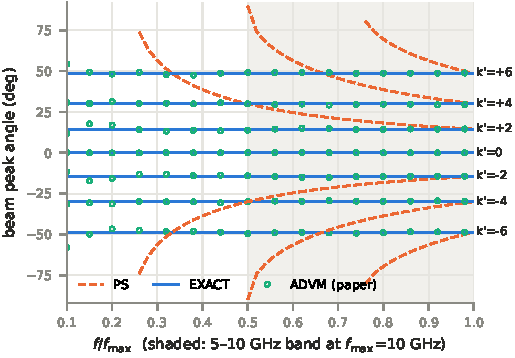
\includegraphics[width=\columnwidth]{../results/figs/F1_peak_vs_freq.pdf}\caption{Beam peak angle versus normalized frequency for $k'\in\{-6,\dots,6\}$. PS (dashed) squints and leaves visible space at low frequency; the TTD (EXACT) beams are flat; ADVM markers stay near EXACT in the band but drift at low frequency.}\label{fig:f1}\end{figure}

Over the course band the squint spread is 60.0$^\circ$ for PS, 1.0e-12$^\circ$ for EXACT and 1.69$^\circ$ for the paper's ADVM (Fig.~\ref{fig:f1}, Table~\ref{tab:methods}). EXACT is squint-free to numerical precision; ADVM exceeds the 0.5$^\circ$ squint-free threshold. Worst-case pointing errors are 60.0$^\circ$ (PS), 6.9e-13$^\circ$ (EXACT) and 1.12$^\circ$ (ADVM). Over the full sweep $f/f_{\max}\in[0.1,1]$ the ADVM pointing error grows to 9.45$^\circ$.

\begin{figure}[!t]\centering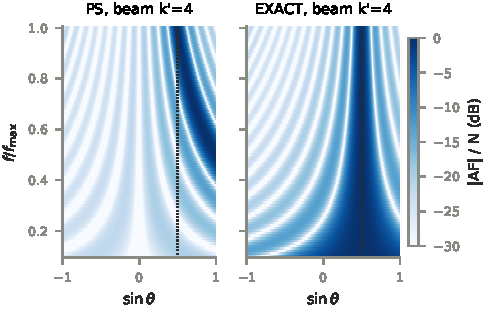
\includegraphics[width=\columnwidth]{../results/figs/F3_heatmap_PS_vs_EXACT.pdf}\caption{$|AF|$ of beam $k'=4$ over $\sin\theta$ and $f/f_{\max}$. PS: tilted ridge (squint). EXACT: vertical ridge at the target (dotted).}\label{fig:f3}\end{figure}

\subsection{Replication of paper Fig.~3}

\begin{figure}[!t]\centering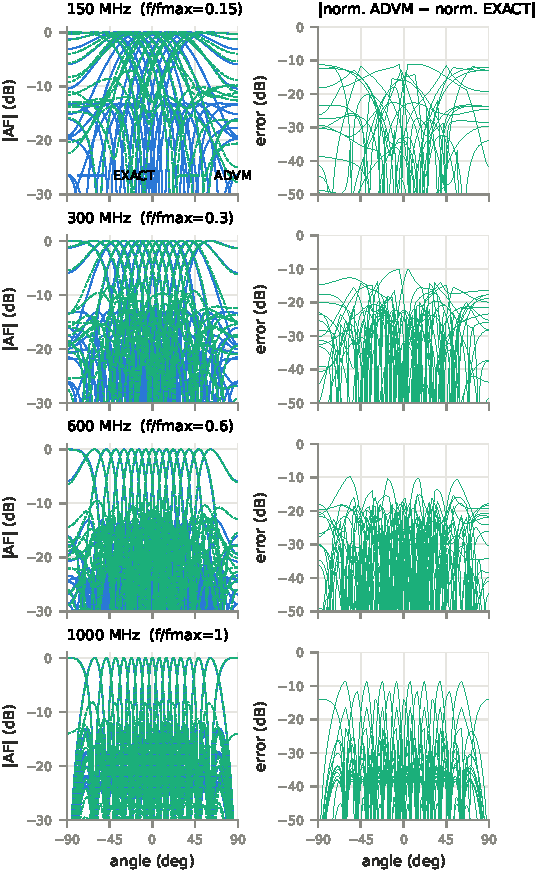
\includegraphics[width=\columnwidth]{../results/figs/F2_paper_fig3_replication.pdf}\caption{All 16 beams at 150, 300, 600 and 1000~MHz ($f_{\max}=1$~GHz). Left: EXACT (solid) vs ADVM (dashed), each beam normalized to 0~dB. Right: magnitude of the difference of the normalized patterns.}\label{fig:f2}\end{figure}

Fig.~\ref{fig:f2} reproduces the paper\textquotesingle s Fig.~3 setup. The ADVM main lobes track EXACT, while the error concentrates in the sidelobe region. The largest normalized-pattern error is -11.1~dB, -10.0~dB, -9.6~dB, -8.5~dB at 150, 300, 600 and 1000~MHz, respectively, and the worst SLL degradation relative to EXACT is 6.8~dB, 5.4~dB, 4.2~dB, 5.0~dB.

\subsection{Complexity}

\begin{figure}[!t]\centering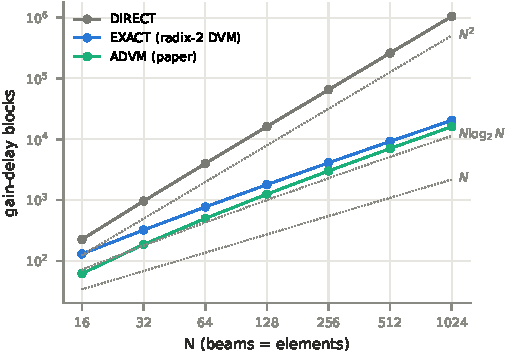
\includegraphics[width=\columnwidth]{../results/figs/F5_complexity.pdf}\caption{Gain-delay blocks counted on the implemented factorizations, with $N^2$, $N\log_2N$ and $N$ reference slopes.}\label{fig:f5}\end{figure}

\begin{table}[!t]\centering\caption{Gain-delay blocks (instrumented) vs.\ paper; area/power reduction (\emph{estimate, proportional model}: area and power $\propto$ gain-delay count)}\label{tab:cx}

\setlength{\tabcolsep}{3pt}\begin{tabular}{rrrrrrr}\hline

$N$ & DIRECT & EXACT & ADVM & Lemma~3.2 & vs DIR. & vs EXACT \\ \hline

16 & 225 & 130 & 62 & 62 & 72.4\% & 52.3\% \\

32 & 961 & 322 & 186 & 186 & 80.6\% & 42.2\% \\

64 & 3969 & 770 & 498 & 498 & 87.5\% & 35.3\% \\

128 & 16129 & 1794 & 1250 & 1250 & 92.2\% & 30.3\% \\

256 & 65025 & 4098 & 3010 & 3010 & 95.4\% & 26.5\% \\

512 & 261121 & 9218 & 7042 & 7042 & 97.3\% & 23.6\% \\

1024 & 1046529 & 20482 & 16130 & 16130 & 98.5\% & 21.2\% \\

\hline\end{tabular}\end{table}

Counting non-trivial multiplications directly on the sparse factors that the code executes reproduces the paper\textquotesingle s Lemma~3.2 for ADVM, its Table~1 counts for the radix-2 DVM, and $(N-1)^2$ for DIRECT at every $N$ (Table~\ref{tab:cx}). At $N=16$ the ADVM needs 62 gain-delay blocks (0 gains, 30 delays, 32 pre-computed anti-causal terms), a 52.3\% reduction versus EXACT and 72.4\% versus DIRECT; at $N=1024$ the reductions are 21.2\% and 98.5\%. The price is adders: at $N=16$ ADVM uses 414 complex additions versus 320 for EXACT. The symmetric-steering pre-delays add $N-1$ delays to every DVM method (not included above).

\subsection{Scalability of the 16-beam building block}

\begin{table}[!t]\centering\caption{ADVM vs EXACT for $N=16,32,64$ (recursion on $\hat{F}_{32}$)}\label{tab:scale}

\setlength{\tabcolsep}{3pt}\begin{tabular}{rrrrrr}\hline

$N$ & $f/f_{\max}$ & patt.\ err (dB) & point.\ err ($^\circ$) & $\Delta$SLL (dB) & rel.\ spec.\ err \\ \hline

16 & 0.15 & -11.1 & 5.27 & 6.8 & 0.300 \\

16 & 0.3 & -10.0 & 1.50 & 5.4 & 0.369 \\

16 & 0.6 & -9.6 & 0.55 & 4.2 & 0.472 \\

16 & 1 & -8.5 & 0.18 & 5.0 & 0.420 \\

32 & 0.15 & -10.1 & 3.58 & 6.5 & 0.328 \\

32 & 0.3 & -11.1 & 0.75 & 4.8 & 0.392 \\

32 & 0.6 & -11.0 & 0.38 & 3.3 & 0.520 \\

32 & 1 & -8.3 & 0.17 & 5.0 & 0.707 \\

64 & 0.15 & -11.3 & 2.76 & 6.4 & 0.316 \\

64 & 0.3 & -12.6 & 0.54 & 5.3 & 0.457 \\

64 & 0.6 & -11.8 & 0.29 & 3.5 & 0.548 \\

64 & 1 & -10.2 & 0.06 & 3.1 & 0.632 \\

\hline\end{tabular}\end{table}

Table~\ref{tab:scale} applies the same ADFT building block recursively for $N=32$ and $64$. The pointing error at a given $f/f_{\max}$ does not grow with $N$, but the relative spectral-norm error stays of order $10^{-1}$ (for $N=16$ it ranges from 0.25 to 0.69 over the sweep).

\subsection{Approximation order (ADVM-b, our extension)}

\begin{figure}[!t]\centering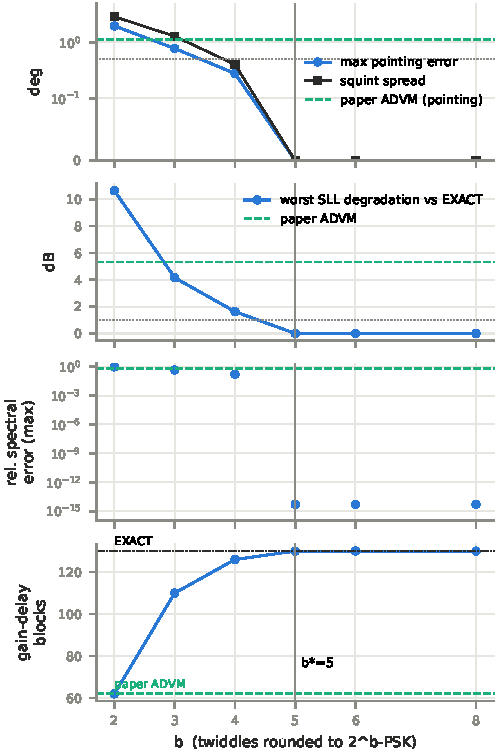
\includegraphics[width=\columnwidth]{../results/figs/F4_bsweep.pdf}\caption{ADVM-b (our extension): twiddles rounded to $2^b$-PSK. Dashed: paper ADVM. Dotted: pass thresholds. Bottom: gain-delay blocks at $N=16$.}\label{fig:f4}\end{figure}

As a separate experiment that is \emph{not} part of the paper, we rounded every twiddle of the exact radix-2 transform to the nearest $2^b$-PSK phase (Fig.~\ref{fig:f4}). The smallest order meeting all three criteria is $b^*=5$. This result is trivial rather than a trade-off: for $N=16$ every twiddle of the 32-point DFT already lies on the 32-PSK grid, so $b\ge5$ is EXACT and costs as much (130 blocks). The informative point is $b=4$ (126 blocks): squint spread 0.40$^\circ$ and pointing error 0.28$^\circ$ pass, but the SLL loss of 1.63~dB fails the 1~dB limit. At the paper\textquotesingle s gain-delay budget (62, i.e.\ $b=2$), rounding is worse than the paper\textquotesingle s ADFT (SLL loss 10.6~dB vs 5.3~dB).

\subsection{Summary of methods}

\begin{figure}[!t]\centering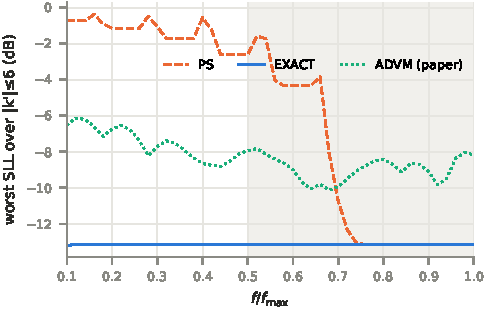
\includegraphics[width=\columnwidth]{../results/figs/F6_sll_vs_freq.pdf}\caption{Worst sidelobe level over beams $|k'|\le6$ versus frequency.}\label{fig:f6}\end{figure}

\begin{table}[!t]\centering\caption{Methods $\times$ metrics, $N=16$, course band (worst case over $|k'|\le6$)}\label{tab:methods}

\setlength{\tabcolsep}{2pt}\begin{tabular}{lrrrrrrc}\hline

Method & squint & point. & gain var. & SLL & $\Delta$SLL & GD & pass \\

 & ($^\circ$) & ($^\circ$) & (dB) & (dB) & (dB) & blocks & \\ \hline

PS & 60.00 & 60.00 & 17.49 & -1.59 & 11.56 & n/a & no \\

EXACT & 0.00 & 0.00 & 0.00 & -13.15 & 0.00 & 130 & yes \\

ADVM & 1.69 & 1.12 & 3.51 & -7.82 & 5.32 & 62 & no \\

ADVM-b (b=2) & 2.89 & 1.97 & 4.28 & -2.51 & 10.64 & 62 & no \\

ADVM-b (b=3) & 1.29 & 0.78 & 1.63 & -8.99 & 4.16 & 110 & no \\

ADVM-b (b=4) & 0.40 & 0.28 & 0.39 & -11.52 & 1.63 & 126 & no \\

ADVM-b (b=5) & 0.00 & 0.00 & 0.00 & -13.15 & 0.00 & 130 & yes \\

ADVM-b (b=6) & 0.00 & 0.00 & 0.00 & -13.15 & 0.00 & 130 & yes \\

ADVM-b (b=8) & 0.00 & 0.00 & 0.00 & -13.15 & 0.00 & 130 & yes \\

\hline\end{tabular}\end{table}

\section{Discussion and Limitations}

\begin{enumerate}

\item \emph{The paper\textquotesingle s ADVM does not meet our criteria.} It halves the gain-delay count at $N=16$ but loses up to 5.3~dB of sidelobe level in the course band (7.0~dB over the full sweep), has 3.5~dB peak-gain variation and 1.69$^\circ$ residual squint. The paper reports a 1--2~dB SLL penalty. We could not reconcile this; one possible cause is the dB convention of the paper\textquotesingle s Fig.~4, where the EXACT sidelobes appear well above the -13.1~dB we obtain for a uniform 16-element array. We did not verify this. The thresholds were fixed before running and were not changed.

\item Multiplication by $\pm j$ is treated as free. In hardware this assumes an ideal wideband $90^\circ$ element (hybrid coupler or Hilbert transformer), which itself has finite bandwidth and error.

\item All delays are ideal: no waveguide or transmission-line dispersion, loss, mismatch, or quantization of the delay values, and the antenna elements are isotropic with no mutual coupling. The results are array-factor computations, not full-wave or measured data.

\item Area and power figures are an \emph{estimate from a proportional model} (area, power $\propto$ gain-delay count, following the paper). Adders, routing and the anti-causal latency are not costed; ADVM needs more adders than EXACT.

\item ADVM-b is our own extension and is not from the paper. For $N=16$ it only reproduces EXACT once $b\ge5$, so it offers no cheaper squint-free design point at this size.

\item The paper\textquotesingle s Fig.~3/4 beams lie on one side of broadside and its element spacing is not stated. We steer symmetrically about broadside, so the replication matches the paper\textquotesingle s set-up and trends, not its exact beam angles.

\end{enumerate}


\section{Physical Significance for the Array}\label{sec:phys}

\begin{figure}[!t]\centering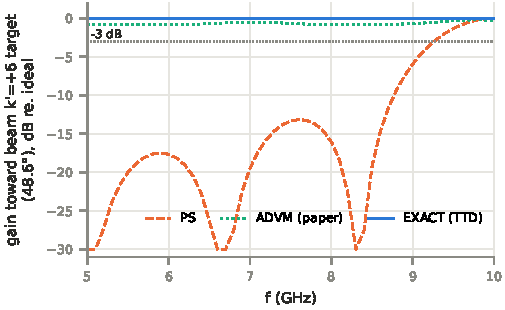
\includegraphics[width=\columnwidth]{../results/figs/F8_gain_at_target.pdf}
\caption{Normalized beamforming gain $|w^{H}a(\theta_k)|^2/(\lVert w\rVert^2 N)$ toward the intended direction of beam $k'=+6$ ($48.6^\circ$), $N=16$. 0~dB is the ideal coherent gain of the array. Values below $-30$~dB (pattern nulls) are clipped.}\label{fig:f8}\end{figure}

\begin{table}[!t]\centering
\caption{What a user at each beam's target angle receives, 5--10~GHz, inner beams $|k'|\le6$}\label{tab:phys}
\setlength{\tabcolsep}{3pt}
\begin{tabular}{lccc}\hline
 & PS & EXACT & ADVM \\ \hline
Loss of band-averaged gain (dB) & 3.9 & 0.0 & 0.7 \\
Band within 3~dB of ideal (\%) & 41 & 100 & 100 \\
\quad worst single beam (\%) & 16 & 100 & 100 \\
Link capacity vs.\ ideal, 20~dB SNR (\%) & 60 & 100 & 97 \\
Delay lines / total length, air (m) & -- & 30 / 2.3 & 30 / 2.3 \\ \hline
\end{tabular}\end{table}

The squint numbers of Sec.~\ref{sec:hw} and before translate into link quality as follows. Fig.~\ref{fig:f8} shows the gain a receiver at a fixed target angle sees as the frequency changes. With phase shifters, the beam swings past the receiver, and the gain stays more than 13~dB below ideal from 5 to about 8.6~GHz, with nulls at about 5, 6.6 and 8.3~GHz. With TTD the gain stays at 0~dB at every frequency. Averaged over the 12 inner beams (Table~\ref{tab:phys}), the phase-shifter array is within 3~dB of ideal for only 41\% of the octave (16\% for the worst beam). Its Shannon capacity $\log_2(1+\mathrm{SNR}\cdot g)$, averaged over the band, is about 60\% of the TTD array's at a nominal 20~dB SNR. ADVM loses 0.7~dB on average and keeps 97\% of the capacity. Its residual squint costs little gain toward the target, but its higher sidelobes (Table~\ref{tab:methods}) raise interference between beams.

The benefit to the array, therefore, is wideband multi-beam operation without squint, and the factorization is what makes it buildable. The direct TTD network needs 225 delay lines and 27~m of line. The exact fast DVM needs 30 lines and 2.3~m (1.1~m in stripline), and the advantage grows as $N^2$ versus $N\log N$ with array size. The dispersion study (Fig.~\ref{fig:f7}) adds a practical constraint: the delay lines must be TEM (stripline, microstrip, coax). Waveguide dispersion brings back $14^\circ$--$33^\circ$ of squint.

These are array-factor results with isotropic elements and ideal, lossless components. Insertion loss of the cascaded passive network, coupler bandwidth and element patterns are not included.

\section{Future Work}
\begin{enumerate}
\item \emph{Realism:} add line loss, the finite bandwidth and phase error of the $90^\circ$/$180^\circ$ hybrids, and element patterns, and check whether ADVM's hardware saving survives.
\item \emph{Better approximations:} search for an approximate DFT that keeps squint below $0.5^\circ$ and sidelobe loss below 1~dB at a lower cost than the exact fast DVM. Our twiddle-rounding variant (ADVM-b) reaches this only when it becomes the exact FFT.
\item \emph{Toward hardware:} circuit-level simulation or a prototype of the $N=16$ network in stripline.
\end{enumerate}

\appendix
\section*{Appendix: Algorithms of~\cite{perera2025}}
% Algorithms 1-4 of Perera et al., IEEE Access 13 (2025) 94488, transcribed as printed.
% Requires \usepackage{algorithm} and \usepackage{algpseudocode}.
\begin{algorithm}[!t]
\caption{$\mathit{Asdvm}$: $y = M\hat{A}_N z$}\label{alg:asdvm}
\begin{algorithmic}[1]
\Require $N=2^r\ (r\ge4)$, $M=2N$, $\alpha\in\mathbb{C}$ with $|\alpha|=1$, $z\in\mathbb{C}^N$ or $\mathbb{R}^N$, $c\in\mathbb{C}^M$
\Ensure $y = M\hat{A}_N z$
\Function{Asdvm}{$z, N$}
  \If{$N = 16$}
    \State $y \gets \Call{Asdvm16}{z, N}$
  \EndIf
  \If{$N \ge 32$}
    \State $u_1 \gets \hat{D}_N\, z$
    \State $u_2 \gets J\, u_1$
    \State $v_1 \gets \Call{Adft}{u_2, M}$
    \State $v_2 \gets \breve{D}_M\, v_1$
    \State $y_1 \gets \Call{Aidft}{v_2, M}$
    \State $y_2 \gets J^{T} y_1$
    \State $y \gets \hat{D}_N\, y_2$
  \EndIf
  \State \Return $y$
\EndFunction
\end{algorithmic}
\end{algorithm}

\begin{algorithm}[!t]
\caption{$\mathit{Asdvm16}$: $y = M\hat{A}_{16} z$}\label{alg:asdvm16}
\begin{algorithmic}[1]
\Require $N=16$, $M=2N$, $z\in\mathbb{C}^N$ or $\mathbb{R}^N$
\Ensure $y = M\hat{A}_{16} z$
\Function{Asdvm16}{$z, N$}
  \If{$N = 16$}
    \State $w_1 \gets \hat{D}_N\, z$
    \State $w_2 \gets J\, w_1$
    \State $w_3 \gets \hat{F}_M\, w_2$ \Comment{$\hat{F}_{32}=S_4S_3S_2S_1S_0$}
    \State $w_4 \gets \breve{D}_M\, w_3$
    \State $w_5 \gets \hat{F}^{*}_M\, w_4$ \Comment{$\hat{F}^{*}_{32}=S_0^TS_1^TS_2^TS_3^TS_4^{*}$}
    \State $w_6 \gets J^{T} w_5$
    \State $y \gets \hat{D}_N\, w_6$
  \EndIf
  \State \Return $y$
\EndFunction
\end{algorithmic}
\end{algorithm}

\begin{algorithm}[!t]
\caption{$\mathit{Adft}$: $v_1 = \hat{F}_M u_2$}\label{alg:adft}
\begin{algorithmic}[1]
\Require $M=2^{r_1}\ (r_1\ge5)$, $M_1=M/2$, $u_2\in\mathbb{C}^M$
\Ensure $v_1 = \hat{F}_M u_2$
\Function{Adft}{$u_2, M$}
  \If{$M = 32$}
    \State $v_1 \gets \hat{F}_{32}\, u_2$
  \EndIf
  \If{$M \ge 64$}
    \State $p \gets H_M\, u_2$
    \State $a_1 \gets \Call{Adft}{p(1\!:\!M_1), M_1}$
    \State $a_2 \gets \Call{Adft}{p(M_1\!+\!1\!:\!M), M_1}$
    \State $v_1 \gets P_M^{T}\,[a_1^T\ a_2^T]^T$
  \EndIf
  \State \Return $v_1$
\EndFunction
\end{algorithmic}
\end{algorithm}

\begin{algorithm}[!t]
\caption{$\mathit{Aidft}$: $y_1 = \hat{F}^{*}_M v_2$}\label{alg:aidft}
\begin{algorithmic}[1]
\Require $M=2^{r_1}\ (r_1\ge5)$, $M_1=M/2$, $v_2\in\mathbb{C}^M$
\Ensure $y_1 = \hat{F}^{*}_M v_2$
\Function{Aidft}{$v_2, M$}
  \If{$M = 32$}
    \State $y_1 \gets \hat{F}^{*}_{32}\, v_2$
  \EndIf
  \If{$M \ge 64$}
    \State $q \gets P_M\, v_2$
    \State $b_1 \gets \Call{Aidft}{q(1\!:\!M_1), M_1}$
    \State $b_2 \gets \Call{Aidft}{q(M_1\!+\!1\!:\!M), M_1}$
    \State $y_1 \gets H^{*}_M\,[b_1^T\ b_2^T]^T$
  \EndIf
  \State \Return $y_1$
\EndFunction
\end{algorithmic}
\end{algorithm}


\begin{thebibliography}{2}
\bibitem{perera2025}
S.~M. Perera, L.~Lingsch, A.~Tuztas, and A.~Madanayake, ``A fast true time-delay wideband multi-beam beamforming algorithm based on a 16-beam approximate-DVM,'' \emph{IEEE Access}, vol.~13, pp.~94488--94507, 2025, doi: 10.1109/ACCESS.2025.3573930.
\bibitem{perera2022}
S.~M. Perera, L.~Lingsch, A.~Madanayake, S.~Mandal, and N.~Mastronardi, ``A fast DVM algorithm for wideband time-delay multi-beam beamformers,'' \emph{IEEE Trans. Signal Process.}, vol.~70, pp.~5913--5925, 2022.
\end{thebibliography}

\end{document}
